\documentclass[a4j]{jarticle}
\usepackage{amsmath}
\usepackage{ascmac}
\usepackage{amssymb}
\usepackage{enumerate}
\usepackage{multicol}
\usepackage{framed}
\usepackage{fancyhdr}
\usepackage{latexsym}
\usepackage{indent}
\usepackage{cases}
\usepackage[dvips]{graphics}
\allowdisplaybreaks
\pagestyle{fancy}
\lhead{}
\chead{}
\rhead{東京大学前期$1975$年$3$番}
\begin{document}
%分数関係


\def\tfrac#1#2{{\textstyle\frac{#1}{#2}}} %数式中で文中表示の分数を使う時


%Σ関係

\def\dsum#1#2{{\displaystyle\sum_{#1}^{#2}}} %文中で数式表示のΣを使う時


%ベクトル関係


\def\vector#1{\overrightarrow{#1}}  %ベクトルを表現したいとき(aベクトルを表現するときは\ver
\def\norm#1{|\overrightarrow{#1}|} %ベクトルの絶対値
\def\vtwo#1#2{ \left(%
      \begin{array}{c}%
      #1 \\%
      #2 \\%
      \end{array}%
      \right) }                        %2次元ベクトル成分表示
      
      \def\vthree#1#2#3{ \left(
      \begin{array}{c}
      #1 \\
      #2 \\
      #3 \\
      \end{array}
      \right) }                        %3次元ベクトル成分表示



%数列関係


\def\an#1{\verb|{|$#1$\verb|}|}


%極限関係

\def\limit#1#2{\stackrel{#1 \to #2}{\longrightarrow}}   %等式変形からの極限
\def\dlim#1#2{{\displaystyle \lim_{#1\to#2}}} %文中で数式表示の極限を使う



%積分関係

\def\dint#1#2{{\displaystyle \int_{#1}^{#2}}} %文中で数式表示の積分を使う時

\def\ne{\nearrow}
\def\se{\searrow}
\def\nw{\nwarrow}
\def\ne{\nearrow}


%便利なやつ

\def\case#1#2{%
 \[\left\{%
 \begin{array}{l}%
 #1 \\%
 #2%
 \end{array}%
 \right.\] }                           %場合分け
 
\def\1{$\cos\theta=c$,$\sin\theta=s$とおく.}  %cs表示を与える前書きシータ
\def\2{$\cos t=c$,$\sin t=s$とおく.}     %cs表示を与える前書きt
\def\3{$\cos x=c$,$\sin x=s$とおく.}                %cs表示を与える前書きx

\def\fig#1#2#3 {%
\begin{wrapfigure}[#1]{r}{#2 zw}%
\vspace*{-1zh}%
\input{#3}%
\end{wrapfigure} }           %絵の挿入


\def\a{\alpha}   %ギリシャ文字
\def\b{\beta}
\def\g{\gamma}

%問題番号のためのマクロ

\newcounter{nombre} %必須
\renewcommand{\thenombre}{\arabic{nombre}} %任意
\setcounter{nombre}{2} %任意
\newcounter{nombresub}[nombre] %親子関係を定義
\renewcommand{\thenombresub}{\arabic{nombresub}} %任意
\setcounter{nombresub}{0} %任意
\newcommand{\prob}[1][]{\refstepcounter{nombre}#1[問題 \thenombre]}
\newcommand{\probsub}[1][]{\refstepcounter{nombresub}#1(\thenombresub)}


%1-1みたいなカウンタ(todaiとtodaia)
\newcounter{todai}
\setcounter{todai}{0}
\newcounter{todaisub}[todai] 
\setcounter{todaisub}{0} 
\newcommand{\todai}[1][]{\refstepcounter{todai}#1 \thetodai-\thetodaisub}
\newcommand{\todaib}[1][]{\refstepcounter{todai}#1\refstepcounter{todaisub}#1 {\bf [問題 \thetodai.\thetodaisub]}}
\newcommand{\todaia}[1][]{\refstepcounter{todaisub}#1 {\bf [問題 \thetodai.\thetodaisub]}}


     \begin{oframed}
     直線$x+y=4$に第一象限において接する放物線$y=-ax^2+bx$がある.この放物線と$x$軸の正の部分とで囲まれる図形の面積が最大とな
     る時の$a$,$b$の値とその場合の面積を求めよ.
     \end{oframed}

\setlength{\columnseprule}{0.4pt}
\begin{multicols}{2}
{\bf[解]} $a\not=0$である.まず,直線の式で$x,y>0$であるから,$0<x<4$となる.方程式から$y$を消去した
     \begin{align*}
     4-x=-ax^2+bx \Longleftrightarrow ax^2-(b+1)x+4=0
     \end{align*}
が$0<x<4$に重解を持つ.判別式$D$として
     \begin{align*}
     \left\{
          \begin{array}{l}
          D=0 \\
          0<\cfrac{b+1}{2a}<4
         \end{array}
    \right.\Longleftrightarrow
    \left\{
          \begin{array}{l}
          (b+1)^2=16a \\
          0<\cfrac{b+1}{2a}<4
         \end{array}
    \right.
     \end{align*}
第一式から$a>0$であるから,($\because a\not=0$)
    \begin{align}
    &\left\{
          \begin{array}{l}
          (b+1)^2=16a \\
          0<b+1<8a
         \end{array}
    \right. \nonumber\\
    \Longleftrightarrow
    &\left\{
          \begin{array}{l}
          (b+1)^2=16a \\
          0<b+1<\cfrac{(b+1)^2}{2}
         \end{array}
    \right. \nonumber\\
    \Longleftrightarrow
    &\left\{
          \begin{array}{l}
          (b+1)^2=16a \\
          1<b
         \end{array}
    \right.  \label{1}
     \end{align}
この時,放物線の概形は下図のようになる.
     \begin{center}
     \scalebox{0.5}{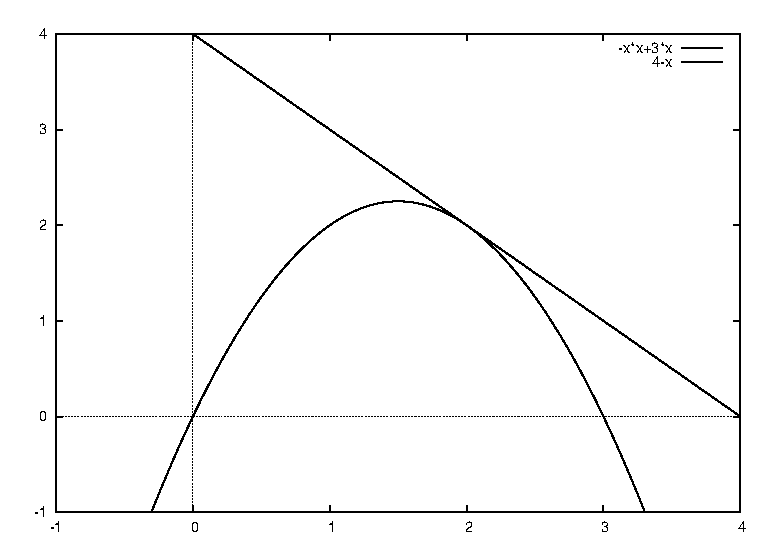
\includegraphics{ut-75-3.eps}}
     \end{center}
     
 \\
     
     題意の面積$S$として
     \begin{align*}
     S&=\int_0^{b/a}(-ax^2+bx)dx \\
     &=\frac{a}{6}\left(\frac{b}{a}\right)^3=\frac{b^3}{6a^2}
     \end{align*}
である.以下\eqref{1}の下でこの最大値を考えれば良い.\eqref{1}を代入して
     \begin{align}
     S&=\frac{b^3}{6}\frac{16^2}{(b+1)^4} \nonumber\\
     &=\frac{128}{3}\frac{b^3}{(b+1)^4}\label{2} 
     \end{align}
ここで$b>1$の時,AM-GMから
     \begin{align*}
     \frac{3b^3}{(b+1)^4}&\le\left(\frac{1}{4}\left(\frac{3}{b+1}+3\frac{b}{b+1}\right)\right)^4 \\
     &=\left(\frac{3}{4}\right)^4 \\
     \therefore &\frac{b^3}{(b+1)^4}\le \frac{3^3}{4^4}
     \end{align*}
である.等号成立は$\cfrac{3}{b+1}=\cfrac{b}{b+1}\Longleftrightarrow b=3$の時.これは\eqref{1}を満たす.従って\eqref{2}
に代入して
     \begin{align*}
     &S\le\frac{128}{3}\frac{3^3}{4^4}=\frac{9}{2}
     &\therefore \max S=\frac{9}{2}
     \end{align*}
である.等号成立は\eqref{1}から$(a,b)=(1,3)$の時である.$\cdots$(答)
     
     
\newpage
\end{multicols}
\end{document}